\subsection{Supervised Machine Learning Models}
\label{subsec:supervised_machine_learning}

This section presents several \emph{Supervised Machine Learning} models that are used in the paper.

Models are separated into two different groups depending on how they describe the input and output variables.

\begin{description}
	\item[Continuous Models] take a matrix $X \in \mathbb{R}^{n \times f}$ and a vector $y \in \mathbb{R}^n$ of the same height where each element represents the features corresponding to some user and its real value, respectively. Its accuracy is measured according to some function of the result of the regression $\ypred$ and $\ytrue = y$.
	\item[Categorical Models] take a matrix $X \in \mathbb{R}^{n \times f}$ and a vector $y \in \mathbb{S}^n$, for some set of \emph{Categories} $\mathbb{S}$, and predicts the correct category each of the users in $y$ belongs to. Its accuracy is measured according to several metrics which are explained in Section~\ref{subsec:mlmetrics}.
\end{description}

\subsubsection{Linear Regression}
\label{subsec:linearregression}

A \emph{Linear Regression} is an approach for modeling the relationship between the matrix $X$ and the real vector $y$. While it's possible to predict many variables in what's known as the \emph{Multivariate Linear Regression}~\cite{multivariate1979}, this thesis will focus in the single-dimensional variant.

The regression assumes that the relationship between the sum of some linear combination of the elements of $X$ and $y$ is itself linear. This combination is represented by the variable $\beta$, and the relationship is represented through an unobserved random vector $\varepsilon$ as the \emph{Error Term}.

The model takes the form of Equation~\ref{eq:linearregression}.

\begin{equation}
\label{eq:linearregression}
	y = X \beta + \varepsilon
\end{equation}

where

\begin{equation*}
\begin{gathered}
	X = \begin{pmatrix} x_1^T \\ x_2^T \\ \vdots \\ x_n^T \end{pmatrix} =
	\begin{pmatrix}
		1 & x_{1 1} & \cdots & x_{1 f} \\
		1 & x_{2 1} & \cdots & x_{2 f} \\
		\vdots & \vdots & \ddots & \vdots \\
		1 & x_{n 1} & \cdots & x_{n f} \\
	\end{pmatrix} \\
	y = \begin{pmatrix} y_1 \\ y_2 \\ \vdots \\ y_n \end{pmatrix}, \;
	\beta = \begin{pmatrix} \beta_0 \\ \beta_1 \\ \vdots \\ \beta_f \end{pmatrix}, \;
	\varepsilon = \begin{pmatrix} \varepsilon_1 \\ \varepsilon_2 \\ \vdots \\ \varepsilon_n \end{pmatrix}
\end{gathered}
\end{equation*}

$\beta$ is a vector with size $f + 1$, where $\beta_0$ is called the \emph{Constant Term}. The statistical estimation and inference focuses in this variable, as two different models of \emph{Linear Regression} will give different results where this parameter is different~\cite{yan2009linear}.

$\varepsilon_i$ is called the \emph{Error Term} or \emph{Noise}. The variable captures the factors which influence the vector $y$ other than the matrix $X$ and the \emph{Constant Term} $\beta$. The relationship between $\varepsilon$ and those variables and knowing whether they are correlated is important in the formulation of an \emph{Linear Regression} model~\cite{yan2009linear}.

This model makes several assumptions about the data.

\begin{description}
	\item[Weak Exogenety] implies than the variables in $X$ can be treated as fixed values, rather than random variables.
	\item[Linearity] implies that the mean of the response variable is a linear combination of the parameters.
	\item[Homoscedasticity] implies that different response variables have the same \emph{Variance} in their errors. While this is almost never true in practice, since variables tend to vary over a large scale, the data is usually \emph{Standardised} so that this is true.
	\item[Independence of errors] implies that the errors in response variables are uncorrelated with each other, even if they are statistically dependent.
	\item[Lack of multicollinearity] implies that the matrix $X$ must have full column rank; there can't be two perfectly correlated input variables. In this case there won't be a unique solution for the vector $\beta$.
\end{description}

There are many ways of effectively calculating the optimal \emph{Lineal Regression} for a particular pair $\left< X, y \right>$. One of them is using the \textbf{Least Squares Estimation}, which can be solved through the \emph{Least Squares Principle}.

\begin{equation}
\label{eq:leastsquaresprinciple}
	\hat{\beta} = \operatorname{argmin}_\beta \left[ {\left( y - X \beta \right)}^T \left( y - X \beta \right)\right]
\end{equation}

Where $\hat{\beta}^T = \left( b_0, b_1, \dots, b_{k - 1} \right)$, a k-dimensional vector of the estimations of the regression coefficients.

Assuming $\left( X^T X \right)$ is a non-singular matrix, the \emph{Least Squares Estimation} of $\beta$ can for the model in Equation~\ref{eq:linearregression} can be found from Equation~\ref{eq:linearsquares}~\cite{yan2009linear}.

\begin{equation}
\label{eq:linearsquares}
	\hat{\beta} = {\left( X^T X \right)}^{-1} X^T y
\end{equation}

Additionally, Equation~\ref{eq:linearsquares} presents an unbiased estimator of $\beta$~\cite{yan2009linear}.

\subsubsection{Logistic Regression}
\label{subsec:logisticregression}

The \emph{Logistic Regression}, also referred to as the \emph{Logit Model}~\cite{freedman2009statistical} is a regression model similar to the \emph{Linear Regression}, with the particularity that the \emph{Dependent Variable} $y$ is categorical. While it's possible to calculate the variable for sets of categories of several finite sizes (when it's referred to as a \emph{Multinomial Logistic Regression}~\cite{greene_econometric_2011}) or even for ordered sets of categories (an \emph{Ordinal Logistic Regression}~\cite{mccullagh1980ordinal}), this thesis will focus on the case where $y \in {\left\{ 0, 1 \right\}}^n$, that is, each variable in $y$ is binary.

The model uses the results of a \emph{Linear Regression} on the data $\left< X, y \right>$, where coefficients that solve Equation~\ref{eq:linearregression} are found. The result of that regression is a real value, which is normalized using a function $f : \mathbb{R} \rightarrow \left[ 0, 1 \right]$, whose result is considered the probability that the result of some element is $1$.

A commonly used function for $f$ is the \emph{Logistic Function} $\sigma : \mathbb{R} \rightarrow \left[ 0, 1 \right]$, defined in Equation~\ref{eq:logisticfunction} and plot in Figure~\ref{fig:sigmoid}.

\begin{equation}
\label{eq:logisticfunction}
\sigma \left( t \right) = \frac{e^t}{e^t + 1} = \frac{1}{1 + e^{-t}}
\end{equation}

\begin{figure}
\centering
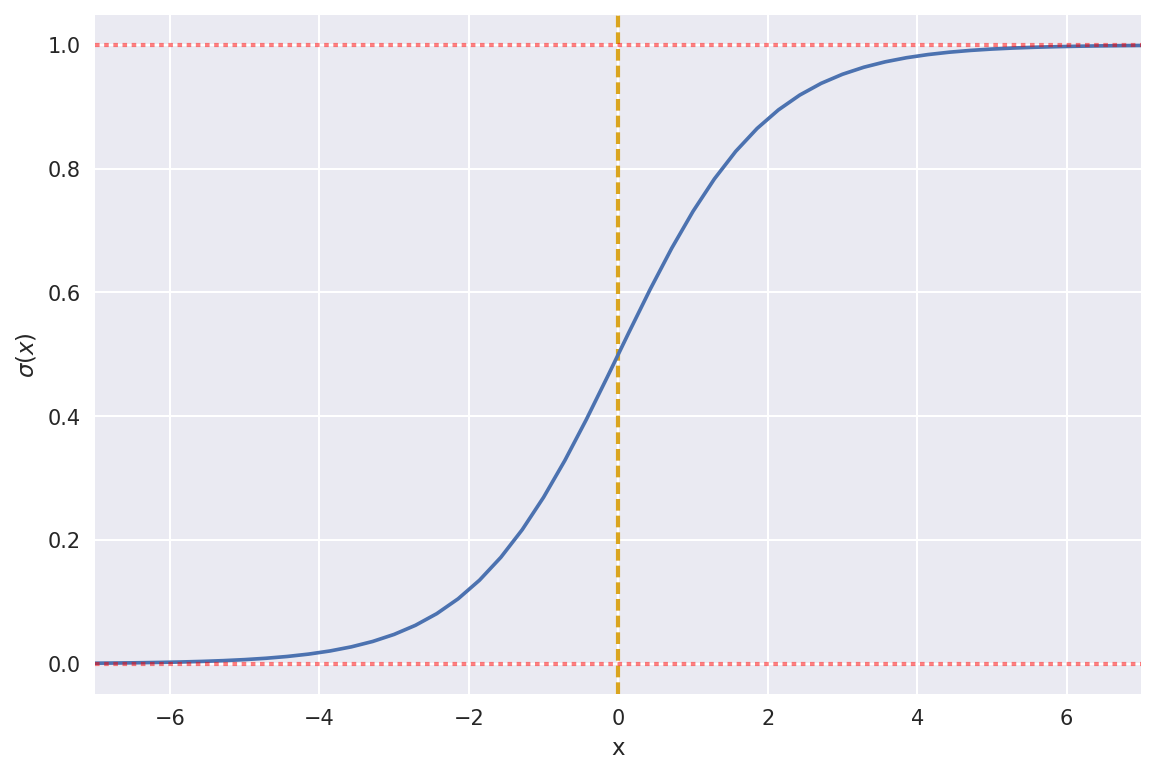
\includegraphics[width=.75\textwidth]{figures/sigmoid.png}
\caption{The standard logistic sigmoid function $y = \sigma(x)$}
\label{fig:sigmoid}
\end{figure}

This probability is used for estimating the value of $y$, namely as defined in Equation~\ref{eq:probit}.

\begin{equation}
\label{eq:probit}
\begin{aligned}
	P \left( y_i = 1 \mid X \right) &= \sigma \left( X_i \beta \right) \\
	P \left( y_i = 0 \mid X \right) &= 1 - \sigma \left( X_i \beta \right)
\end{aligned}
\end{equation}

The inverse of the \emph{Logistic Function}, referred to as the \emph{Logit Function}, gives the logarithm of the \emph{Odds} of a certain element belonging to some category.

\begin{equation}
\label{eq:logit}
	\logit \left( x \right) = \log \left( \frac{\sigma \left( x \right)}{1 - \sigma \left( x \right)} \right)
\end{equation}

The logit model says that the vector $y$ is independent given the matrix $X$~\cite{freedman2009statistical}, and can be considered as inverse of the probability defined in Equation~\ref{eq:probit}.

\begin{equation}
\label{eq:prob_logit}
	\logit P \left( y_i = 1 \mid X \right) = X_i \beta
\end{equation}

The regression is usually calculated using \emph{Maximum Likelihood Estimation}~\cite{fan2008liblinear} and, unlike the estimation of the \emph{Linear Regression} presented in Section~\ref{subsec:linearregression}, it's not possible to find a closed form expression of the coefficients that maximize the value of the likelihood function. Instead, the iterative \emph{Newton's Method} is used.

The exact formulas used to ensure fast and correct conversed used in this thesis are the ones present in \texttt{LIBLINEAR}, which is presented in~\cite{hsiastudy}.

\subsubsection{Decision Trees}
\label{subsec:decisiontrees}

A \emph{Decision Tree} is a decision support tool that uses a tree of decisions and their possible consequencs, influding change event outcomes. They are commonly used in decision analysis to help identify the most optimal strategy to reach a goal.

In the context of \emph{Machine Learning}, it can be used as a supervised predictive model which matches properties about the list of features $X$ to the likeliest cagegory $y$~\cite{oded2008decisiontrees}. In the binary case, which is the focus of this thesis,

\subsubsection{Random Forest}
\label{subsec:randomforest}
\todo{Add Random Forest}

